%Fiber Optik (Arsitektur Komputer)
%Kelas : D4 TI 1B
%Khadijah Hasanah Putri Harahap 1174022
%Liyana Majdah Rahma 1174039
%Luthfi Muhammad Nabil 1174035
%Nisrina Aulia Firdaus 1174098
%Salwaa Tania 1174047
%Septia Rahayu 1174044
%Diana Satima Gistivani 1154018

\section{Fiber Optic}
\begin{flushleft}
Fiber Optic merupakan sebuah kabel tembus pandang berbahan kaca atau plastik yang halus dan kecil yang digunakan untuk mentransmisikan sinyal cahaya dari satu tempat ke tempat lain, Sumber cahaya dari Fiber Optic biasanya menggunakan cahaya Laser atau LED. Ukuran diameter dari kabel ini kurang lebih sekitar 125 mikrometer atau sekitar 1/8 mm. Kabel Fiber Optic sendiri biasa dipakai dalam kepentingan Jaringan telepon atau Koneksi Internet.
\end{flushleft}
\begin{flushleft}
Gelombang cahaya pada kabel Fiber Optic dipantulkan dari satu ujung ke ujung yang lain tanpa menggunakan perantara apapun, radius dari pantulan cahaya Fiber Optic bisa mencapai 50 Kilometer sedangkan jika memakai perantara seperti repeater dapat mencapai 100 Kilometer. kabel Fiber Optic memiliki daya pantul cahaya yang sangat tinggi sehingga membuat cahaya pada kabel tidak mudah meredup atau melemah dibagian tengah kabel. 
\end{flushleft}
\section{Sejarah Fiber Optic}
\begin{flushleft}
Kabel Fiber Optic mulai dibuat dan dikembangkan pada tahun 1970, saat Ilmuwan dari Corning Glass Works yaitu Donald Keck, Peter Schultz, dan Robert Maurer melaporkan penemuan Fiber Optic yang memenuhi syarat yang ditentukan oleh Kao dan Hockham. Mereka dapat mengurangi kerugian cahaya sampai kurang dari 20 decibels per kilometer menggunakan Kaca murni yang dibuat terdiri dari gabungan silika. Dilanjutkan pada tahun 1972, tim ini menemukan Kaca yang mampu mengurangi kerugian cahaya sampai hanya 4 decibels per kilometer. Pada tahun 1970, Morton Panish dan Izuo Hayashi dari Bell Laboratories mendemonstrasikan laser semikonduktor yang dapat dioperasikan pada temperatur ruang. Dengan adanya penemuan dari kedua tim inilah Kabel Fiber Optik mulai berkembang.
\end{flushleft}
\begin{flushleft}
Pada tahun 1977 Perusahaan telepon mulai menggunakan Fiber Optic dengan mengganti sistem kawat tembaga menjadi jalur Fiber Optic. Perusahaan telepon sendiri menggunakan Fiber Optic diseluruh sistem mereka sebagai sistem komunikasi jarak jauh antar kota. Dengan adanya pemakaian yang meledak membuat Industri Fiber Optic semakin mengalami keuntungan. Pada tahun 1980, sebuah perusahaan AT\&T membuka jaringan Fiber Optic yang menghubungkan kota antara Boston dan Washington D.C. di Amerika. Perusahaan elektronik sendiri mulai mencoba memainkan peranan dalam mendalami riset Fiber Optic.
\end{flushleft}
\begin{flushleft}
Fiber Optic mulai bersifat lebih mudah dikembangkan dan lebih efisien penggunaannya dari masa ke masa, seperti halnya pada tahun 1987 David Payne dari Universitas Southampton yang mengenalkan optical amplifiers yang dicampur oleh elemen erbium yang dapat menaikkan sinyal cahaya tanpa harus dikonversikan ke dalam energi listrik terlebih dahulu juga pada tahun 1991 yaitu Emmanuel Desurvire dan David Payne yang mengintegrasikan kabel Fiber Optic dengan Optical Amplifiers yang membuat informasi sampai 100 kali lebih cepat daripada kabel dengan penguat elektronik.
\end{flushleft}
\begin{flushleft}
Penggunaan Kabel Fiber Optic mulai sangat efektif diantaranya dengan munculnya sebuah kabel jenis TPC-5 yang merupakan kabel Fiber Optic yang menggunakan penguat optik. Kabel ini sudah menghubungkan antara negara - negara yang sudah bekerjasama, mulai dari San Luis Obispo, California, ke Guam, Hawaii, dan Miyazaki dan kabel ini dapat menangani sekitar 320.000 panggilan telepon. dengan berkembangnya kabel Fiber Optic membuat seluruh dunia dapat terhubung dengan mudah.Munculnya Link Around the Globe membuat jaringan kabel Fiber Optic terpanjang dan terluas di seluruh dunia yang telah menyediakan infrastruktur untuk generasi internet terbaru.
\end{flushleft}
\section{Karateristik Fiber Optic}
\begin{flushleft}
\begin{figure}[ht]
\centerline{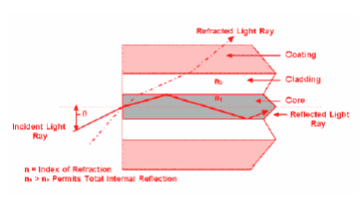
\includegraphics[width=0.6\textwidth]{figures/skemafiber.png}}
\caption{Skema dari Kabel Fiber Optic}
\label{Skema Fiber Optic}
\end{figure}
Fiber Optic memberikan dampak yang besar dalam dunia pengiriman sebuah informasi, mulai dari koneksi lokal sampai koneksi antar benua. Fiber optic sendiri merupakan suatu media pengiriman yang sangat pesat perkembangannya. Data yang dikirimkan pada kabel Fiber Optic sendiri berupa analog dan digital. Sistematis pengiriman data berasal dari listrik yang kemudian diubah ke optic oleh sumber cahaya berupa cahaya LED. Seperti pada gambar \ref{Skema Fiber Optic}, Kabel Fiber Optic memiliki beberapa Struktur data. Struktur data dari Fiber Optic diantaranya sebagai berikut : 
\begin{enumerate}
\item Core (Inti)\\ Berfungsi untuk menuntukan cahaya yang merambat dari ujung satu ke ujung lainnya. Core sendiri memiliki beberapa ciri - ciri diantaranya : \\ 
	\begin{itemize}
	\item Terbuat dari kuarsa yang berkualitas tinggi
	\item Merupakan dari bagian Fiber Optic
	\end{itemize}
\item Cladding (Lapisan)\\ Berfungsi untuk memantulkan cahaya agar dapat merambat ke ujung satunya. Cladding memiliki beberapa ciri - ciri diantaranya : \\
	\begin{itemize}
	\item Terbuat dari kaca dengan index bias yang lebih rendah dari Core (Inti).
	\item Hubungan antara Cladding dan Core mempengaruhi perambatan cahaya pada core.
	\end{itemize}
\item Coating (Pelindung) \\ Berfungsi sebagai pelindung kabel. Coating memiliki beberapa ciri - ciri diantaranya : \\
	\begin{itemize}
	\item Memiliki bahan dari plastik.
	\item Berfungsi untuk melindungi Fiber Optic dari segala kerusakan.
	\end{itemize}
\end{enumerate}
\end{flushleft}
\begin{flushleft}
Indeks bias pada Core harus lebih besar dari indesk bias pada Cladding. Bahan dari Core sendiri tidak harus terbuat dari bahan yang sejenis dengan Cladding melainkan bisa dibuat dengan menggunakan bahan selembar senar transparan yang berfungsi sebagai core dan Cladding udara dan lain sebagainya. Pada bidang komunikasi Optik, bahan Fiber Optic dibuat menggunakan bahan silica yang murni pada core maupun cladding. Untuk membedakan indeks bias core dan cladding, bahan silica murni diberi campuran yang memiliki kadar berbeda untuk setiap core dan cladding. Bentuk pemampang kabel Fiber Optic yang berbentuk lingkaran ukuran diameternya sekitar 125 mikrometer atau sekitar 1/8 mm.
\begin{figure}[ht]
\centerline{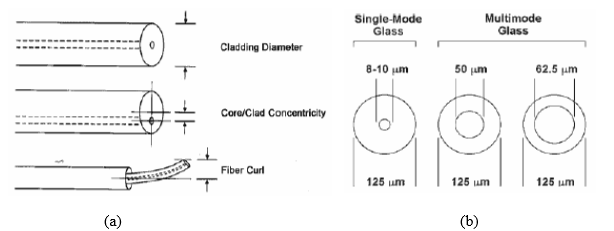
\includegraphics[width=1\textwidth]{figures/sizeanddiameter.png}}
\caption{(a). Diameter Cladding, Core, dan Fiber Curl  (b). Ukuran Fiber Optic}
\label{Skema Fiber Optic}
\end{figure}
\end{flushleft}
\begin{flushleft}
Bentuk penampang dari core Fiber Optic adalah berbentuk ellips dan berbentuk lingkaran. Tipe kabel yang umum digunakan dalam kebutuhan telekomunikasi dapat dilihat dari ukuran diameter dari Core. Tipe dari kabel tersebut diantaranya mode tunggal (Single mode/mono mode) dan mode jamak (multi mode). Dari kedua kabel tersebut memiliki banyak perbedaan dimana kabel fiber optic single mode lebih mahal dibandingkan kabel fiber optic multi mode, dimana kabel fiber optic single mode lebih efektif dibandingkan dengan kabel fiber optic multi mode. Jika dilihat dari distribusi indeks bias core, kabel fiber optic memiliki beberapa jenis diantaranya : 
\begin{enumerate}
\item Step Index Multimode \\ Merupakan index bias core konstan yang memiliki ukuran diameter 50 mikrometer dan dilapisi oleh cladding yang sangat tipis. jenis ini dapat digunakan untuk transmisi jarak pendek dan data bit rate rendah.
\item Graded Index Multimode \\ Merupakan cahaya yang dapat merambat karena difraksi yang terjadi pada core sehingga cahaya dapat merambat sejajar dengan sumbu serat
\item Step Index Singlemode \\ Memiliki diameter core yang lebih kecil dibandingkan dengan ukuran cladding
\end{enumerate}
\end{flushleft}
%tambahindarisiniya
\section{Manfaat Fiber Optic}
\subsection 
Teknologi serat optik (fiber optic) ini akan memberikan kemungkinan yang lebih baik bagi jaringan telekomunikasi, terutama dalam hal telekomunikasi data. 
Serat optik (fiber optic) adalah salah satu media transmisi yang dapat menyalurkan informasi dengan kapasitas besar dengan tingkat keandalan (performance) yang tinggi. 
Beda dengan media transmisi lain, pada teknologi serat optik (fiber optic) ini, gelombang pembawanya tak lagi merupakan gelombang elektromagnetik (microwave) atau listrik, 
tapi merupakan sinar atau cahaya laser. 
Kabel serat optik (fiber optic) mampu melayani transfer data dengan kecepatan tinggi dalam waktu yang relatif singkat dan bentuk fisi yang relatif kecil dan ringan.

